%!TEX root = ../thesis.tex
\chapter{Introduction}
\label{chap:introduction}

%
This capstone project does the following several things coded in Python:
it first sets market data retrieval using Unicorn data feed and parses market data in json format to store market data for backtesting in SQLite database; then implements trading logic; sets up Python Client/Server communication and multi-threading and implements real-time feed to simulate real trade; finally displays trading analysis and PnL on web dashboard. The program has to run in order as described. The program design is also shown in flow chart Figure 1.1.

\begin{figure}
\centering
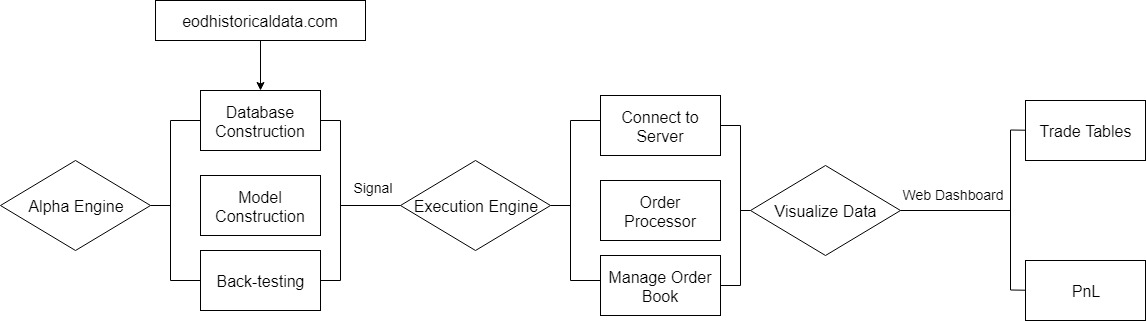
\includegraphics[scale=0.35]{introduction/images/flowchart.jpg}
\caption{Program Design}
\label{fig:flow}
\end{figure}

%
The server is a multi-thread application which coordinates among all the client applications. Its main purposes are 1) messaging among all the participants, 2) maintain a market participant list, and the list of stocks traded by participants, and 3) generate a consolidated order book for all the participants. The client application, also a multi-threading application in network-oriented environment, will communicate with the server. Each application will implement required messages in json format. 

%
Moreover, 1) The sender and receiver threads will support TCP/IP protocol and through Internet sockets;
2) The sender and receiver threads must achieve data synchronization using event and queue;
3) the application will handle direct market data feeds in json format for historical and real-time data from eodhistoricaldata.com;
4) the application will have an integrated database for data persistence. The database we use is sqlite3. We implement tables and SQL statements for our own model buildup, as well as back testing.
5) We will implement a trading model.
6) We manage our own order books and calculate P/L.

%
The trading model is a pairs trading model on stocks in SP500. We use machine learning techniques in selecting pairs. Specifically, we use PCA to reduce dimensions and then DBSCAN clustering to group stocks. We then identify pairs within clusters to implement dollar neutral Bollinger Band pairs trading strategy. Finally, we construct a portfolio with pairs equally weighted. We achieve a 2.5 Sharpe ratio backtested in 2018. However, we can potentially lose money when we trade in simulated market using client/server infrastructure we built.

%
We proceed as follows. In Chapter 2: Background, we provide some backgrounds in pairs trading model and machine learning techniques we used. Chapter 3: Data, we describe how we retrieve, parse and store data into database. In Chapter 4: Trading Model, we describe our trading logic, how we train, build and backtest our model. In Chapter 5: Client/Server, we provide details of client server infrastructure and how they communicate. In Chapter 6: Simulated Trade, we explain how we implement trading strategy to trade in client/server infrastructure. In Chapter 7: Performance Analysis, we show our performance of backtest and simulated trade results and how we move the visualization to web dashboard using flask. At last, we have Chapter 8: Conclusion and appendix where source codes will be provided.